\documentclass[11pt]{article}
\usepackage{amssymb}
\usepackage{amsmath}
\usepackage{a4wide}
\usepackage[dutch]{babel}
\usepackage{graphicx}
\usepackage{pstricks}
\usepackage{wrapfig}

%\parindent=0mm

%\newcommand{\andspaceNL}{\hspace{10mm} {\rm en} \hspace{10mm}}
\newcommand{\RR}{\ensuremath{\mathbb{R}}}
\newcommand{\ZZ}{\ensuremath{\mathbb{Z}}}
\newcommand{\QQ}{\ensuremath{\mathbb{Q}}}
\newcommand{\NN}{\ensuremath{\mathbb{N}}}
\newcommand{\CC}{\ensuremath{\mathbb{C}}}
\newcommand{\rarr}{\rightarrow}
\newcommand{\ds}{\displaystyle}
\newcommand{\Rnulplus}{\ensuremath{\mathbb{R}_0^+}}
\DeclareMathOperator{\bgsin}{bgsin}
\DeclareMathOperator{\bgtan}{bgtan}
\begin{document}
{\Huge\textbf{Voorkennisles 1}}
\section{Goniometrische functies}

\subsection{Goniometrische cirkel}

\begin{wrapfigure}{r}{0pt}
\psset{unit=0.25 cm}

%\noindent
  \begin{pspicture}(-7,-6)(7,7)

%cos-as
  \psline{->}(-6,0)(7,0)

%sin-as
  \psline{->}(0,-6)(0,7)

\pscircle[linewidth=0.3 pt](0,0){5}
\psarc[linewidth=0.9pt](0,0){5}{0}{60}

%hoeken
\psline[linewidth=0.5 pt](3,5.196152423)(0,0)
  \pscircle*(2.5,4.330127019){0.1}
  \uput{0.2}[0] (2.5,4.330127019){$P$}
  \psarc(0,0){1}{0}{60}
  \uput{1.2}[30] (0,0){$\alpha$}

%labels cos
  \uput{0.2}[-90] (5,0){\psframebox*{$1$}}

%labels sin
  \uput{0.2}[180] (0,5){\psframebox*{$1$}}
  \uput{0.2}[225] (0,0){\psframebox*{$0$}}

\end{pspicture}
\end{wrapfigure}
Een goniometrische cirkel is een cirkel met als middelpunt $(0,0)$
en met straal 1. Met elke hoek $\alpha$ kan een punt $P$ van de
goniometrische cirkel geassocieerd worden. Hiertoe laat men het
eerste been van de hoek samenvallen met de positieve $x$-as. Het
tweede been snijdt de goniometrische cirkel in het punt $P$. De hoek
is positief indien die in tegenwijzerzin gemeten wordt vanaf de
$x$-as. Dus elk punt van de cirkel kan gezien worden als de
voorstelling van een hoek. Hoeken worden gemeten in graden of in
radialen. De eenheid radialen is zo gekozen dat de lengte van de
cirkelboog van de goniometrische cirkel tussen de twee benen de hoek
uitgedrukt in radialen geeft. De omtrek van een cirkel met straal
$1$ is $2 \pi $. Het verband tussen graden en radialen wordt dus
gegeven door $2 \pi = 360^\circ $. Een rechte hoek bv. is $90^\circ$
of $\ds \frac{\pi}{2}$ radialen.

\psset{unit=0.04\textwidth} \noindent
  \begin{pspicture}(-8,-7)(8,6)
\pscircle[linewidth=0.3 pt](0,0){5}
%cos-as
    \psline{->}(-7,0)(7,0)

%sin-as
    \psline{->}(0,-7)(0,6)

%hoeken
  \psline[linewidth=0.5 pt](2.5,4.330127019)(-2.5,-4.330127019)
  \psline[linewidth=0.5 pt](4.330127019,2.5)(-4.330127019,-2.5)
  \psline[linewidth=0.5 pt](3.535533906,3.535533906)(-3.535533906,-3.535533906)

  \psline[linewidth=0.5 pt](-2.5,4.330127019)(2.5,-4.330127019)
  \psline[linewidth=0.5 pt](-4.330127019,2.5)(4.330127019,-2.5)
  \psline[linewidth=0.5 pt](-3.535533906,3.535533906)(3.535533906,-3.535533906)

%labels hoeken
 \uput{0.05}[210](4.330127019,2.5){\psframebox*{$\frac{\pi}{6}$}}
 \uput{0.05}[225](3.535533906,3.535533906){\psframebox*{$\frac{\pi}{4}$}}
 \uput{0.05}[240](2.5,4.330127019){\psframebox*{$\frac{\pi}{3}$}}
 \uput{0.05}[-45](0,5){\psframebox*{$\frac{\pi}{2}$}}
 \uput{0.05}[300](-2.5,4.330127019){\psframebox*{$\frac{2\pi}{3}$}}
 \uput{0.05}[315](-3.535533906,3.535533906){\psframebox*{$\frac{3\pi}{4}$}}
 \uput{0.05}[330](-4.330127019,2.5){\psframebox*{$\frac{5\pi}{6}$}}
 \uput{0.05}[180](-5,0){\psframebox*{$\pi$}}
 \uput{0.05}[210](-4.330127019,-2.5){\psframebox*{$\frac{7\pi}{6}$}}
 \uput{0.05}[225](-3.535533906,-3.535533906){\psframebox*{$\frac{5\pi}{4}$}}
 \uput{0.05}[240](-2.5,-4.330127019){\psframebox*{$\frac{4\pi}{3}$}}
 \uput{0.05}[270](0,-5){\psframebox*{$\frac{3\pi}{2}$}}
 \uput{0.05}[120](2.5,-4.330127019){\psframebox*{$\frac{-\pi}{3}$}}
 \uput{0.05}[135](3.535533906,-3.535533906){\psframebox*{$\frac{-\pi}{4}$}}
 \uput{0.05}[-45](3.535533906,-3.535533906){\psframebox*{$\frac{7\pi}{4}$}}
 \uput{0.05}[150](4.330127019,-2.5){\psframebox*{$\frac{-\pi}{6}$}}

%hoeken
\pscircle*(4.330127019,2.5){0.1}
\pscircle*(3.535533906,3.535533906){0.1}
\pscircle*(2.5,4.330127019){0.1} \pscircle*(0,5){0.1}
\pscircle*(-2.5,4.330127019){0.1}
\pscircle*(-3.535533906,3.535533906){0.1}
\pscircle*(-4.330127019,2.5){0.1} \pscircle*(-5,0){0.1}
\pscircle*(-4.330127019,-2.5){0.1}
\pscircle*(-3.535533906,-3.535533906){0.1}
\pscircle*(-2.5,-4.330127019){0.1} \pscircle*(0,-5){0.1}
\pscircle*(2.5,-4.330127019){0.1}
\pscircle*(3.535533906,-3.535533906){0.1}
\pscircle*(4.330127019,-2.5){0.1}

\end{pspicture}

\begin{itemize}
\item Hoeveel radialen is $120^\circ$?
\item Hoeveel graden is 1 rad?
%\item

%Wat is de lengte van de cirkelboog op onderstaande figuur?

% \psset{unit=0.25 cm}

%\noindent
%  \begin{pspicture}(-10,-6)(10,7)
%\pscircle[linewidth=0.3 pt](0,0){5}
%cos-as
%  \psline{->}(-6,0)(7,0)

%sin-as
%  \psline{->}(0,-6)(0,7)

%hoeken
%\pswedge[linewidth=1pt](0,0){5}{90}{225}
%\psline[linewidth=0.5 pt](-3.535534,-3.535534)(0,0)
%  \psarc(0,0){1}{90}{225}
%  \uput{1}[135] (0,0){$135^\circ$}

%labels cos
%  \uput{0.2}[-90] (5,0){\psframebox*{$2$}}


%labels sin
 % \uput{0.2}[180] (0,5){\psframebox*{$2$}}
 % \uput{0.2}[225] (0,0){\psframebox*{$0$}}

%\end{pspicture}
\end{itemize}

\subsection{Goniometrische getallen}
De cosinus en sinus van de hoek $\alpha$ zijn gedefinieerd via de
co\"ordinaten van het punt $P$. Stel $(x,y)$ de co\"ordinaten van
$P$ dan geldt $x=\cos \alpha, y=\sin \alpha$. De tangens (afgekort
tan of tg) en de cotangens (afgekort cot, cotg of cotan) zijn
gedefinieerd als
\[\tan \alpha=\frac{\sin \alpha}{\cos \alpha} \hspace{2cm} \cot \alpha=\frac{\cos \alpha}{\sin \alpha}\]
en kunnen eveneens aangeduid worden op de goniometrische cirkel.
\psset{unit=0.45 cm}

\noindent
  \begin{pspicture}(-10,-6)(10,10)

%cos-as
  \psline{-|*}(-6,0)(2.5,0)
  \psline{-|*}(2.5,0)(5,0)
  \psline{->}(5,0)(10,0)

%sin-as
  \psline{-|*}(0,-6)(0,4.330127019)
  \psline{-|*}(0,4.330127019)(0,5)
  \psline{->}(0,5)(0,10)

%cotan-as
%  \psline{->}(-10,5)(10,5)
  \psline{-|*}(-6,5) (2.8867513,5)
  \psline{->}(2.8867513,5)(10,5)


%tan-as
%  \psline{->}(5,-10)(5,10)
  \psline{-|*}(5,-6) (5,8.660254038)
  \psline{->}(5,8.660254038)(5,10)

%hoeken

  \psline[linewidth=0.5 pt](5,8.660254038)(0,0)
  \pscircle*(2.5,4.330127019){0.1}
  \uput{0.2}[0] (2.5,4.330127019){$P$}
  \psarc(0,0){1}{0}{60}
  \uput{1.2}[30] (0,0){$\alpha$}

%stippellijnen

  \psline[linewidth=0.5 pt,linestyle=dotted,dotsep=1.5pt](2.5,4.330127019)(2.5,0)
  \psline[linewidth=0.5 pt,linestyle=dotted,dotsep=1.5pt](2.5,4.330127019)(0,4.330127019)

%labels cos

  \uput{0.2}[-90] (2.5,0){\psframebox*{$\cos \alpha$}}
  \uput{0.2}[-90] (5,0){\psframebox*{$1$}}
%  \uput{0.2}[-90] (0,0){\psframebox*{$0$}}

%labels sin
  \uput{0.2}[180] (0,4.330127019){\psframebox*{$\sin \alpha$}}
  \uput{0.2}[180] (0,5){\psframebox*{$1$}}
%  \uput{0.2}[180] (0,-5){\psframebox*{$-1$}}
  \uput{0.2}[225] (0,0){\psframebox*{$0$}}



%labels cotan
%  \uput{0.2}[90] (0,5) {\psframebox*{0}}
%  \uput{0.2}[90] (5,5){\psframebox*{1}}
  \uput{0.2}[90] (2.886751346,5){\psframebox*{$\cot\alpha$}}

%labels tan

%  \uput{0.2}[0] (5,0) {\psframebox*{0}}
  \uput{0.2}[0] (5,8.660254038){\psframebox*{$\tan \alpha$}}
%  \uput{0.2}[0] (5,5) {\psframebox*{1}}



\pscircle[linewidth=0.3 pt](0,0){5}
  \uput{0.2}[180] (0,5){\psframebox*{$1$}}
  \uput{0.2}[-90] (5,0){\psframebox*{$1$}}

\end{pspicture}

Uit de stelling van Pythagoras volgt meteen dat $\sin^2 \alpha +
\cos^2 \alpha = 1$.
%\begin{itemize}
%\item
%Duid op onderstaande figuur $\sin \alpha, \cos \alpha$ en $\tan
%\alpha$ aan:

%\psset{unit=0.45 cm}

%\noindent
%  \begin{pspicture}(-10,-6)(10,7)

%cos-as
 % \psline{-|*}(-6,0)(4.330127019,0)
 % \psline{-|*}(4.330127019,0)(5,0)
 % \psline{->}(5,0)(10,0)

%sin-as
 % \psline{-|*}(0,-6)(0,2.5)
 % \psline{-|*}(0,2.5)(0,5)
 % \psline{->}(0,5)(0,7)

%cotan-as
 % \psline{-|*}(-6,5) (8.660254038,5)
 % \psline{->}(8.660254038,5)(10,5)


%tan-as
%  \psline{-|*}(5,-6) (5,2.8867513)
 % \psline{->}(5,2.8867513)(5,7)

%hoeken

%  \psline[linewidth=0.5 pt](8.660254038,5)(0,0)
 % \pscircle*(4.330127019,2.5){0.1}

%  \psarc(0,0){1}{30}{90}
%  \uput{1.2}[60] (0,0){$\alpha$}

%stippellijnen

%  \psline[linewidth=0.5 pt,linestyle=dotted,dotsep=1.5pt](4.330127019,2.5)(0,2.5)
%  \psline[linewidth=0.5 pt,linestyle=dotted,dotsep=1.5pt](4.330127019,2.5)(4.330127019,0)

%\pscircle[linewidth=0.3 pt](0,0){5}
 % \uput{0.2}[180] (0,5){\psframebox*{$1$}}
%  \uput{0.2}[-90] (5,0){\psframebox*{$1$}}

%\end{pspicture}

%\end{itemize}
 Enkele veel voorkomende hoeken en hun
goniometrische getallen zijn gegeven in onderstaande tabel.

\begin{center}
\begin{tabular}{|c|c|c|c|c|c|} \hline
$x$      & $0$ & $\frac{\pi}{6}$ & $\frac{\pi}{4}$ & $\frac{\pi}{3}$ & $\frac{\pi}{2}$ \\[5pt] \hline
  &  & & &  &  \\
$\sin x$ & $0$ & $\frac{1}{2}$  & $\frac{1}{2} \sqrt{2}$ & $\frac{1}{2}\sqrt{3}$ & $1$ \\[10pt]
$\cos x$ & $1$ & $\frac{1}{2} \sqrt{3}$ & $\frac{1}{2} \sqrt{2}$ & $\frac{1}{2}$ & $0$ \\[10pt]
$\tan x$ & $0$ & $\frac{1}{3} \sqrt{3}$ & $1$ & $\sqrt{3}$ & $-$ \\[5pt] \hline
\end{tabular}
\end{center}

\noindent {Voor een rechthoekige driehoek met rechthoekszijden $x$ en $y$, schuine zijde $r$ en  $\theta$ de hoek ingesloten tussen $x$ en $r$, geldt:

\parbox{10 cm}
{
\begin{align*}
\cos \theta= &\frac{x}{r}\\
\sin \theta= &\frac{y}{r}\\
\tan \theta =\frac{\sin \theta}{\cos \theta}=&\frac{y}{x}
\end{align*}
} \hfill
  \parbox{5 cm}{ \begin{pspicture}(0,-1)(5,3)
  \psline (0,0) (4,0) (4,3)(0,0)
  \rput[t](2,-0.2){$x$}
  \rput[l](4.2,1.5){$y$}
  \rput[r](1.8,1.5){$r$}
  \psarc[linewidth=0.5 pt](0,0){0.8}{0}{36.8}
  \uput{0.9}[18.4](0,0){$\theta$}
  \uput{0}[90]{90}(4,0){\psline (0.3,0.1)(0.1,0.1)(0.1,0.3)}
  \end{pspicture} }
	
\subsection{Sinus en cosinus functie}
Zie cursus Wiskunde I p 53. Deze functies gebruiken hoeken gemeten
in radialen als argument.
\begin{itemize}
\item Lees volgende waarden af op de goniometrische cirkel:
\begin{itemize}
\item[] $\sin 0= $ \hspace{2cm} $\sin \frac{\pi}{2}=$ \hspace{2cm} $\sin \pi=$ \hspace{2cm} $\sin \frac{ 3 \pi}{2}=$ \hspace{2cm} $\sin 2 \pi=$

\end{itemize}
\item Schets de grafiek van $f(x) = \sin x$
\newpage
\item Geef alle oplossingen van volgende  vergelijkingen
\begin{enumerate}
\item $\sin x = 0$
\vspace{3mm}
\item $\sin x  = 1$
\vspace{3mm}
\item $\ds \sin ( \frac{\pi}{2} x) = 0$
\end{enumerate}
\end{itemize}


\subsection{Verwante hoeken}
Een overzicht vind je op Toledo, onder Studiebegeleiding-Voorkennislessen-LES 1
\begin{itemize}
\item
Wat is het verband tussen $\cos({\frac{5 \pi}{6}})$ en
$\cos({\frac{\pi}{6}})$?
\end{itemize}

\vspace{2.5cm} 

\begin{itemize}
%\item
%Zijn onderstaande uitspraken juist of fout? Gebruik hiervoor
%onderstaande figuur.

%\begin{enumerate}
%\item $\sin(\alpha) = \cos(\frac{\pi}{2} + \alpha)$
%\item $\sin(\alpha) = \cos(\frac{\pi}{2} - \alpha)$
%\item $\sin(\alpha) = - \sin(\frac{\pi}{2} + \alpha)$
%\item $\sin(\alpha) = \cos( - \frac{\pi}{2} + \alpha)$
%\item $\sin(\alpha) = - \sin(- \alpha)$
%\end{enumerate}

% \psset{unit=0.45 cm}

%\noindent
%  \begin{pspicture}(-10,-6)(10,6)

%cos-as
 %   \psline{->}(-6,0)(6,0)

%sin-as
  %\psline{-|*}(0,-6)(0,4.330127019)
  %\psline{-|*}(0,4.330127019)(0,5)
  %\psline{->}(0,5)(0,6)

%hoeken

%  \psline[linewidth=0.5 pt](2.5,4.330127019)(0,0)
%  \pscircle*(2.5,4.330127019){0.1}
%   \psarc(0,0){1}{0}{60}
%  \uput{1.2}[30] (0,0){$\alpha$}

%stippellijnen

 %  \psline[linewidth=0.5 pt,linestyle=dotted,dotsep=1.5pt](2.5,4.330127019)(0,4.330127019)

%labels cos

 %  \uput{0.2}[-90] (5,0){\psframebox*{$1$}}


%labels sin
  %\uput{0.2}[180] (0,4.330127019){\psframebox*{$\sin \alpha$}}
  %\uput{0.2}[180] (0,5){\psframebox*{$1$}}
  %\uput{0.2}[225] (0,0){\psframebox*{$0$}}



%\pscircle[linewidth=0.3 pt](0,0){5}
%  \uput{0.2}[180] (0,5){\psframebox*{$1$}}
%  \uput{0.2}[-90] (5,0){\psframebox*{$1$}}

%\end{pspicture}
\item Geef alle oplossingen van de vergelijking $\sin \alpha = -
\frac{\sqrt 3}{2}$

\psset{unit=0.03\textwidth} \noindent
  \begin{pspicture}(-10,-6)(10,6)

%cos-as
  \psline{->}(-6,0)(6,0)

%sin-as
  \psline{-|*}(0,-6)(0,-5)
  \psline{-|*}(0,-5)(0,-4.330127019)
  \psline{-|*}(0,-4.330127019)(0,-3.535533906)
  \psline{-|*}(0,-3.535533906)(0,-2.5)
  \psline{-|*}(0,-2.5)(0,2.5)
  \psline{-|*}(0,2.5)(0,3.535533906)
  \psline{-|*}(0,3.535533906)(0,4.330127019)
  \psline{-|*}(0,4.330127019)(0,5)
  \psline{->}(0,5)(0,6)

%hoeken

  \psline[linewidth=0.5 pt](2.5,4.330127019)(-2.5,-4.330127019)
    \psline[linewidth=0.5 pt](-2.5,4.330127019)(2.5,-4.330127019)



%stippellijnen

%  \psline[linewidth=0.5 pt,linestyle=dotted,dotsep=1.5pt](2.5,4.330127019)(2.5,-4.330127019)
 % \psline[linewidth=0.5 pt,linestyle=dotted,dotsep=1.5pt](2.5,4.330127019)(-2.5,4.330127019)

%  \psline[linewidth=0.5 pt,linestyle=dotted,dotsep=1.5pt](3.535533906,3.535533906)(3.535533906,-3.535533906)
%  \psline[linewidth=0.5 pt,linestyle=dotted,dotsep=1.5pt](3.535533906,3.535533906)(-3.535533906,3.535533906)

%  \psline[linewidth=0.5 pt,linestyle=dotted,dotsep=1.5pt](4.330127019,2.5)(4.330127019,-2.5)
%  \psline[linewidth=0.5 pt,linestyle=dotted,dotsep=1.5pt](4.330127019,2.5)(-4.330127019,2.5)

%  \psline[linewidth=0.5 pt,linestyle=dotted,dotsep=1.5pt](-2.5,4.330127019)(-2.5,-4.330127019)
%  \psline[linewidth=0.5 pt,linestyle=dotted,dotsep=1.5pt](2.5,-4.330127019)(-2.5,-4.330127019)

%  \psline[linewidth=0.5 pt,linestyle=dotted,dotsep=1.5pt](-3.535533906,3.535533906)(-3.535533906,-3.535533906)
%  \psline[linewidth=0.5 pt,linestyle=dotted,dotsep=1.5pt](3.535533906,-3.535533906)(-3.535533906,-3.535533906)

%  \psline[linewidth=0.5 pt,linestyle=dotted,dotsep=1.5pt](-4.330127019,2.5)(-4.330127019,-2.5)
%  \psline[linewidth=0.5 pt,linestyle=dotted,dotsep=1.5pt](4.330127019,-2.5)(-4.330127019,-2.5)

\pscircle[linewidth=0.3 pt](0,0){5}
  \uput{0.2}[180] (0,5){\psframebox*{$1$}}
  \uput{0.2}[180] (0,-5){\psframebox*{$-1$}}
  \uput{0.2}[-90] (5,0){\psframebox*{$1$}}


%hoeken
\pscircle*(4.330127019,2.5){0.1}
\pscircle*(3.535533906,3.535533906){0.1}
\pscircle*(2.5,4.330127019){0.1} \pscircle*(0,5){0.1}
\pscircle*(-2.5,4.330127019){0.1}
\pscircle*(-3.535533906,3.535533906){0.1}
\pscircle*(-4.330127019,2.5){0.1} \pscircle*(-5,0){0.1}
\pscircle*(-4.330127019,-2.5){0.1}
\pscircle*(-3.535533906,-3.535533906){0.1}
\pscircle*(-2.5,-4.330127019){0.1} \pscircle*(0,-5){0.1}
\pscircle*(2.5,-4.330127019){0.1}
\pscircle*(3.535533906,-3.535533906){0.1}
\pscircle*(4.330127019,-2.5){0.1}

\end{pspicture}
\end{itemize}



\subsection{Goniometrische formules}
Zie cursustekst Wiskunde I p 54. Let hierbij op de gebruikte
notaties: $$(\cos \alpha)^2 \neq \cos (\alpha^2)$$ Wel geldt:
$$(\cos \alpha)^2 = \cos^2 (\alpha)= \cos^2 \alpha$$
Onthou ook dat $\cos 2 \alpha \neq 2 \cos \alpha$. Waaraan is $\cos
2 \alpha$ wel gelijk?
\begin{itemize}
\item Toon aan dat $\displaystyle 1 + \tan^2 \alpha = \frac{1}{\cos^2 \alpha}$ met behulp van de hoofdformule $\sin^2 \alpha + \cos^2
\alpha = 1$
\end{itemize}

\section{Rekenen}
\subsection{Absolute waarde p7}
Voor een re\"eel getal
$a\in \RR$ defini\"eren we de \emph{ absolute waarde} van $a$
als \\$$|a|\overset{def}{=}\displaystyle\ \left\{\begin{array}{rll  } a & \mbox{als}& a \geqslant 0, \\
-a & \mbox{als} & a<0.\\
\end{array}\right.$$
\begin{itemize}
	\item Voorbeelden: $|5|=5,\; |-\pi|=\pi$ en $|1-\sqrt{2}|=\sqrt{2}-1$
	\item Eigenschap: Als $x \in \RR$ en $r>0 $, dan geldt: $|x|<r\qquad \Leftrightarrow
\qquad -r<x<r$
\end{itemize}

\subsection{Eigenschappen ongelijkheden}
 Voor elke $x,y,z \in\RR $ geldt
\begin{enumerate}
\item \label{opt}$x< y \;\Leftrightarrow \;x+z< y+z$.
\item\label{factor} $(x<y $ en $ \displaystyle z>
0)\; \Leftrightarrow \; xz< yz$.
\item \label{neg
factor}$(x< y $ en $ \displaystyle z<0)\; \Leftrightarrow \; xz>
yz$.
\end{enumerate}


\subsubsection*{Een functie toepassen op beide leden van een
ongelijkheid} Enkele voorbeelden:
\begin{enumerate}
\item \label{kwadraat pos}Als $x,y \geqslant 0,$ geldt $ (x< y \;
\Leftrightarrow \; x^{2}< y^{2})$.
\item \label{kwadraat neg}Als $x,y \leqslant 0,$ geldt $ (x<y \; \Leftrightarrow \;
x^{2}> y^{2})$.
\item \label{wortel} Als $x,y \geqslant 0,$ geldt $ (x< y \; \Leftrightarrow \; \sqrt{x}<\sqrt{y}).$

\end{enumerate}


We bekijken de grafiek van de functie met voorschrift $f(x) =x^2:$
\begin{center}

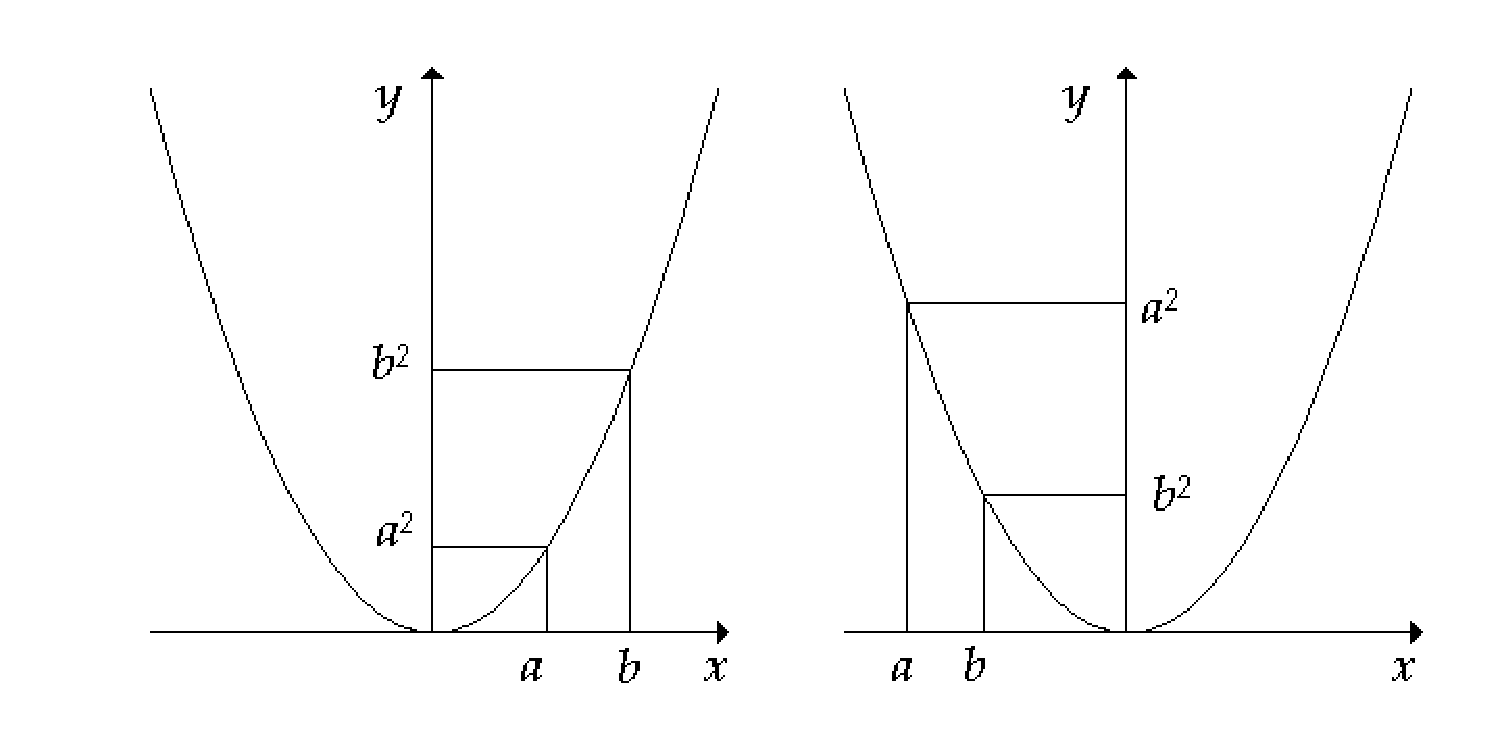
\includegraphics[width=9cm]{parabool2bis.ps}\end{center}

De figuur links illustreert dat
$$\mbox{als }a,b \geqslant 0, \mbox{ dan geldt } a<b\Leftrightarrow
a^2<b^2$$
\\De rechtse figuur  illustreert dat $$\mbox{als }a,b \leqslant 0, \;\mbox{ dan
geldt } \;a<b\Leftrightarrow a^2>b^2$$

Als $a<0<b \;\mbox{ kan je niet weten of }\;a^2<b^2,\; \mbox{ofwel}
\;a^2>b^2$.
%, zoals je op volgende figuren kan inzien.
%\begin{center}
%\includegraphics[width=9cm]{parabool3bis.ps}

%\end{center}

\subsection{Eerste - en tweedegraads veeltermen p25}
\begin{itemize}
\item De grafiek van de functie $f$ met voorschrift $ f(x)= ax+b$ is een rechte met $a$ als richtingsco\"effici\"ent en b als snijpunt met de $y$-as.
De vergelijking van de rechte door $(x_1,y_1)$ en $(x_2,y_2)$ is:
$$y-y_1 = \frac{y_2-y_1}{x_2-x_1} (x-x_1)$$
\item
De grafiek van de functie $f$ met voorschrift $ f(x)= ax^2+bx+c$ met
 $a\neq 0$ is een parabool.
We hebben een bergparabool als $a<0$ en een dalparabool als $a>0$.
\\$D=b^2-4ac$ noemt men de \emph{discriminant}
\begin{itemize}
\item Als $D > 0$ heeft $f$ 2 nulpunten:
$\displaystyle{\frac{-b\pm \sqrt{D}}{2a}}$
\item Als $D = 0$ heeft $f$ 1 nulpunt: $\displaystyle{-\frac{b}{2a}}$
\item Als $D<0$ heeft $f$ geen nulpunten.
\end{itemize}
Als $x_1$ en $x_2$ nulpunten zijn dan geldt: $ax^2+bx+c = a
(x-x_1)(x-x_2)$.
\end{itemize}

\subsection{Ontbinden in factoren}
Een derdegraadsveelterm $f(x) = b x^3+ c x^2+ d x+ e$ ontbinden in
factoren van zo laag mogelijke graad: \begin{itemize} \item Stap 1:
Zoek een nulpunt $a$ van $f(x)$. Dan kunnen we $f(x)$ schrijven als
$f(x) = (x-a) Q(x)$ met $Q(x)$ een tweedegraadsveelterm.
\item Stap 2: Bereken $\ds Q(x) = \frac{f(x)}{x-a}$
\item Stap 3: Ontbind $Q(x)$ verder in factoren indien mogelijk
\end{itemize}
Eig:  Als $b x^3+ c x^2+ d x+ e$, met $b$,$c$, $d$, $e$ gehele
getallen, deelbaar is door $(x-a)$, met $a$ geheel, dan moet $a$ een
deler zijn van de constante term $e$. Indien $f(x)$ geen enkel
geheel nulpunt heeft dan moeten we een benaderingsmethode gebruiken
(zie Hoofdstuk 5)


\subsection{Faculteit en binomiaalco\"effici\"ent}
\begin{itemize}
\item $n! = n.(n-1).(n-2) \ldots  3.2.1$
\item $\displaystyle \left( \begin{array}{c} n \\ k \end{array} \right) = \frac{n!}{k! (n-k)!}$
\end{itemize}

\subsection{Rekenen met breuken}
Zij $a,b,c,d\in \RR$. Er geldt:
\begin{itemize}
\item $\ds{\frac{a}{b}+\frac{c}{d}}=\ds{\frac{ad+cb}{bd}}$ \hspace{3mm}   indien $b,d \neq 0$
\item $\ds{\frac{\frac{a}{b}}{\ c\ }}=\ds{\frac{a}{bc}}$ \hspace{3mm}   indien $b,c \neq 0$
\item $\ds{\frac{a}{\ \frac{b}{c}\ }}=\ds{\frac{ac}{b}}$ \hspace{3mm}   indien $b,c \neq 0$
%\item $\ds{\frac{\frac{a}{b}}{\ \frac{c}{d}\ }}=\ds{\frac{ad}{bc}}$ \hspace{3mm}   indien $b,c,d \neq 0$
\end{itemize}
\subsection{Machten p6}
Zij $x,y>0$ en $m,n\in\RR$. Er geldt:

\begin{itemize}
\item $\ds{x^{m}x^{n}}= \ds{x^{m+n}}$
\item $\ds{\sqrt[n] x = x^{\frac1n}}$
\item
$\ds{\frac{x^{m}}{x^{n}}}= \ds{x^{m-n}}$
\item
$\ds{(xy)^n}=\ds{x^ny^n}$
\item
$\ds{\left(x^{m}\right)^{n}}= \ds{x^{mn}}$

\end{itemize}

\section{Oefeningen}

\begin{enumerate}
\item
 Onderzoek welke $x\in \RR$ voldoen aan
 \begin{enumerate}
\item $\displaystyle |3x-2| < 5$
\item $|3-2x| < 1$
\item  $|\sqrt{x}+3|<9$
\item $\displaystyle \left|  \frac{9 - \sqrt{1+20x}}{10} \right| < 1$
\item  $\displaystyle \left|5-\frac{2}{x}\right|>1$
 
\item $(x+3)(x-2)(x-4) < 0$
\item $\ds \frac{2x+1}{x+3} > 3$
\item $\ds x^2  \geq 3x -2$
\item $y x^2 + x -y = 0$
\item $e^{2x} + e^x -6 = 0$
\item $e^x -4 e^{-x} = 3$
\item $a x^2 + (a^2 - 2) x -2 a = 0$

\end{enumerate}


\item Geef de vergelijking van de rechte door $(2,5)$ en $(3,8)$.
\item Schets de grafiek van $x-2y=-2$.

\item Bepaal het quoti\"ent en de rest van de deling van
\begin{enumerate}
\item $4x^4+x^3+2x+1$ door $2x^2+1$
\item $2 x^3 + x^2 - 8x + 5$ door $x-1$
\item $4x^3+4x^2-5x-3$ door $2x^2 -x -1$
\end{enumerate}
Schrijf ook het verband op dat er bestaat tussen deze veeltermen.
\item Ontbind in factoren van zo laag mogelijke graad.
\begin{enumerate}
\item $f(x) = 2 x^3 + x^2 - 8x + 5$
\item $f(x)=15x^3-37x^2+12x+4$
\item $\displaystyle f(x) = \frac{x(x+1)(2x+1)}{6} + (x+1)^2 $
\end{enumerate}

\item Schrijf zo eenvoudig mogelijk.
\begin{itemize}
\item $\ds{\frac{a-b}{c}-\frac{a-2b}{2c}=}$
\item $\ds{\frac{\frac{a-b}{b}}{1-\frac{a}{b}}=}$
\item $\ds{\frac{1-\frac{a+b}{b}}{\frac{a^{2}}{b}}=}$
%\item $\ds\frac{1+\ds\frac{2}{x-1}}{1-\ds\frac{1}{x+2}}-\ds\frac{1-\ds\frac{3}{x-2}}{1-\ds\frac{2}{x+1}}$
\end{itemize}

\item Vereenvoudig
\begin{itemize}
\item $\ds \frac{(m+4)!}{m!} =$
\item $\left( \begin{array}{c} k+1 \\ k \end{array} \right) =$
\item $\ds \frac{1}{(k+1) (k-1)!} + \frac{1}{(k+1)!} =$
\item $\left( \begin{array}{c} 2k \\ k \end{array} \right) =$
\item $\ds \frac{1}{(k-1)! (n+1)!} + \frac{1}{k! n!} =$
\end{itemize}

\item Los op naar $x$:
\begin{itemize}
\item $\ds x^{\frac32} -3 = 0$
\item $\ds \frac{1}{x} + \frac{1}{b} = \frac{1}{a}$
\end{itemize}

\item Schrijf zo eenvoudig mogelijk ($a>0, b>0, x>0, y>0$).
%Stel $x,y \in \R$ en $a,b \in \Rnul$.
\begin{itemize}
\item $\ds{\frac{\sqrt{a}}{a^{5}}=}$
\item $\ds{\left(x^{6}y^{8}\right)^{-1/2}=}$
\item $\ds{a^{4}b\left(\frac{\sqrt{a^{2}b^{4}}}{ab}\right)^{3}=}$
\end{itemize}

\item Vul aan:
\begin{itemize}
\item $\displaystyle \frac{1}{32} = 2^{...}$  \hspace{2cm}
$\displaystyle 36 \sqrt6 = 6^{...}$ \hspace{2cm} $0.00001 =
10^{...}$
\end{itemize}


\end{enumerate}
\section*{Oplossingen}

\begin{enumerate}
\item
\begin{enumerate}
\item $]-1,\frac73[$
\item $]1 , 2[$
\item $[0,36[$
\item $[ - \frac{1}{20} , 18 [$
\item $]-\infty, 0[\;\cup \;]0, \ds\frac{1}{3}[\;\cup\;
]\ds\frac{1}{2},+\infty[$
\item $]- \infty, -3 [ \;\cup\; ] 2,4[$

\item $]-8,-3[$

\item $]-\infty,1]\;\cup\;[2,+\infty[$

\item $\ds x= \frac{- 1 + \sqrt{1 + 4y^2}}{2y}$  \hspace{5mm} en \hspace{5mm} $\ds x= \frac{-1 - \sqrt{1 + 4y^2}}{2y}$
\item $x = \ln 2$
\item $x = \ln 4$
\item $x = -a$ en $x= \frac{2}{a}$





\end{enumerate}

\item $y=3x-1$
\item

\item \begin{enumerate}
\item
$4x^4+x^3+2x+1=(2x^2+\frac{1}{2}x-1)(2x^2+1)+(\frac{3}{2}x+2)$
\item $2 x^3 + x^2 - 8x + 5 = (x-1)(2x^2+3x-5)$
\item
$4x^3+4x^2-5x-3 =  (2x^2 -x -1)(2x+3)$
\end{enumerate}
\item
\begin{enumerate}
\item $f(x) = (x-1)^2 (2x+5)$
\item $f(x)=(x-2)(3x-2)(5x+1)$
\item $f(x) = \frac16 (x+1)(x+2)(2x+3)$
\end{enumerate}
\item
\begin{itemize}
\item $ \ds \frac{a}{2c}$
\item $-1$
\item $\ds - \frac{1}{a}$
%\item $ \ds \frac{4x+1}{(x-1)(x-2)}$
\end{itemize}
\item
\begin{itemize}
\item $(m+4)(m+3)(m+2)(m+1)$
\item $k+1$
\item $\frac{1}{k!}$
\item $\frac{(2k)!}{k! k!}$
\item $\frac{k+n+1}{ k! (n+1)!}$
\end{itemize}
\item
\begin{itemize}
\item $\ds x = 3^{\frac23}$
\item $\ds x=\frac{ab}{b-a}$
\end{itemize}
\item
\begin{itemize}
\item $\ds a^{-\frac92}$
\item $x^{-3} y^{-4}$
\item $\ds (ab)^4$
\end{itemize}
\end{enumerate}
\end{document}
